% !TEX root=../meca1321-synthesis.tex

\chapter{Écoulements incompressibles établis}
  Un écoulement au profil transversal de vitesse identique peu importe la section est dit établi, soit "complètement développé" et ne peuvent se rencontrer qu'avec des section de passage invariable le long de l'écoulement. Cependant, l'invariabilité de la section ne garanti pas l'établissement du profil de vitesse. Il s'agit d'une condition nécessaire mais non suffisante. Par convention, la direction d'écoulement est $x$.

  \section{Écoulements de Hagen-Poiseuille et de Couette}
      \subsubsection{Écoulements plans}
        Soit un écoulement établi 2D entre deux plaques planes, fixe et séparées de $d=2h$, dit "de Poiseuille". Le système est décrit à la Figure \ref{fig:Poiseuille}. Comme l'écoulement est établi, $u=u(y)$ et donc que $\pdv{u}{x} = 0$, la continuité implique que $\pdv{v}{y} = 0$ et l'intégration implique que $v = v(x)$. Comme $v=0$ aux parois, on conclu que $v = 0$ partout.
        \begin{figure}[h]
          \centering
          % !TEX root = ../meca1321-synthesis.tex
\tikzsetnextfilename{Poiseuille}
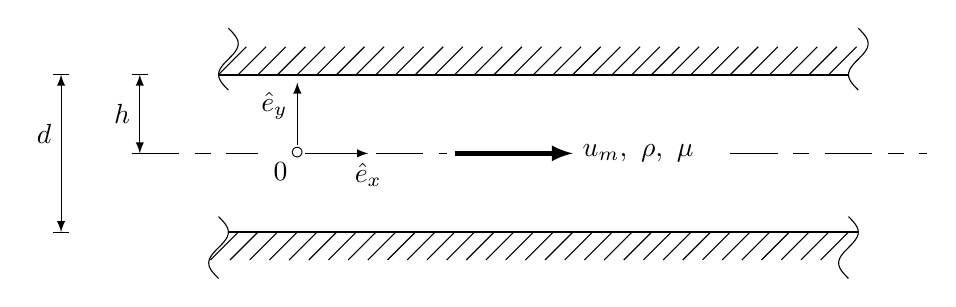
\begin{tikzpicture}
  % Tracé des parois
  \draw [thick] (-4,1) -- (4,1);
  \draw [domain=-pi:pi] plot ({sin(deg(\x))/8-3.875},{((\x+pi/2)/8+1});
  \draw [domain=-pi:pi] plot ({sin(deg(\x))/8+4.125},{((\x+pi/2)/8+1});
  \draw [thick] (-3.875,-1) -- (4.125,-1);
  \draw [domain=-pi:pi] plot ({sin(deg(\x))/8-4},{((\x-pi/2)/8-1});
  \draw [domain=-pi:pi] plot ({sin(deg(\x))/8+4},{((\x-pi/2)/8-1});
  \foreach \i in {0,...,31}
  {
    \pgfmathsetmacro{\x}{(- 4 + \i/4)};
    \draw (\x,1) -- ++(45:0.5);
    \draw (\x+1/4,-1) -- ++(-135:0.5);
  }
  %Repères et autres flèches
  \draw [dash pattern= on 0.6cm off 0.2cm on 0.2cm off 0.2cm] (-5.1,0) -- (-3.5,0);
  \draw [>=latex,<->] (-6,-1) -- (-6,1);
  \draw (-5.1,1) -- ++(0.2,0);
  \draw (-5,0.5) node [left] {$h$};
  \draw [>=latex,<->] (-5,0) -- (-5,1);
  \draw (-6.1,1) -- ++(0.2,0);
  \draw (-6.1,-1) -- ++(0.2,0);
  \draw (-6,0) node [above left] {$d$};
  \draw (-3,0) node {$\circ$};
  \draw (-3,0) node [below left] {$0$};
  \draw [>=latex,->] (-3,0.1) -- (-3,0.9);
  \draw [>=latex,->] (-2.9,0) -- (-2.1,0);
  \draw (-3.0,0.9) node [below left] {$\hat{\vb{e}}_y$};
  \draw (-2.1,0) node [below] {$\hat{\vb{e}}_x$};
  \draw [dash pattern= on 0.6cm off 0.2cm on 0.2cm off 0.2cm] (-2,0) -- (-1.1,0);
  \draw [ultra thick,>=latex,->] (-1,0) -- (0.5,0);
  \draw (0.5,0) node [right] {$u_m,~\rho,~\mu$};
   \draw [dash pattern= on 0.6cm off 0.2cm on 0.2cm off 0.2cm] (2.5,0) -- (5,0);
\end{tikzpicture}

          \caption{Écoulement établi entre deux plaques}
          \label{fig:Poiseuille}
        \end{figure}

        En utilisant la quantité de mouvement (Équation \ref{eq:ConspvT})\footnote{$\rho \vb{g}$ est négligé}, on établit l'équation en $x$ qui donne une équation parabolique après intégration et application des CL en $\pm h$
        \begin{equation}
          \begin{aligned}
            0 &= -\dv{P}{x} + \nu\dv[2]{u}{y} \\ \label{eq:Poiseuille}
            u(y) &= -\dv{P}{x}\frac{h^2}{2\nu} \left(1 - \left(\frac{y}{h}\right)^2\right)
          \end{aligned}
        \end{equation}
        On détermine alors la vitesse maximale obtenue en $y = 0$ et le débit volumique (par unité de profondeur)
        \begin{multicols}{2}
          \begin{equation}
            u_c = -\dv{p}{x} \frac{h^2}{2\mu}
          \end{equation}

          \begin{equation}
            Q = 2\int_0^h u(y)dy = \frac{4}{3} h u_c
          \end{equation}
        \end{multicols}

        La vitesse de débit est définie comme étant le débit volumique divisé par la section
        \begin{equation}
          u_m = \frac{Q}{2h} = \frac{2}{3} u_c
        \end{equation}
        Ce qui permet d'établir que le profil de vitesse est
        \begin{equation}
          u(y) = \frac{3}{2} u_m \left(1-\left(\frac{y}{h}\right)^2\right)
        \end{equation}

        \begin{figure}[h]
          \centering
          \begin{minipage}[c]{0.45\textwidth}
            % !TEX root = meca1321-synthesis.tex
\tikzsetnextfilename{PoiseuilleProfile}
\begin{tikzpicture}[scale=0.8]
  \draw (-4,-3) -- (3,-3);
  \draw (-4,3) -- (3,3);
  \draw (-3,-3) -- (-3,3);
  \foreach \i in {0,...,2}
  {
    \pgfmathsetmacro{\x}{(-3 + \i*3)};
    \draw (\x,-3) -- ++(0,-0.2);
    \draw (\x,-3.2) node [below] {$\i$};
  }
  \draw (-3,0) -- ++(-0.2,0);
  \draw (-3.2,0) node [left] {$0$};
  \draw (-4,-3) node [left] {$-1$};
  \draw (-4,3) node [left] {$1$};
  \draw (1.5,-3.1) node [below] {$u/u_m$};
  \draw (-3.1, 1.5) node [left] {$y/h$};
  \draw [domain=-1:1] plot ({(3/2)*(1-(\x)^(2))*3-3},{\x*3});
\end{tikzpicture}

            \caption{Profil de vitesse pour l'écoulement de Poiseuille entre 2 plaques}
            \label{fig:PoiseuilleProfile}
          \end{minipage}
          \begin{minipage}[c]{0.45\textwidth}
            % !TEX root = meca1321-synthesis.tex
\tikzsetnextfilename{CouetteProfile}
\begin{tikzpicture}[scale=0.8]
  \draw (-4,-3) -- (3,-3);
  \draw (-4,3) -- (3,3);
  \draw (-3,-3) -- (-3,3);
  \foreach \i in {0,...,2}
  {
    \pgfmathsetmacro{\x}{(-3 + \i*3)};
    \draw (\x,-3) -- ++(0,-0.2);
    \draw (\x,-3.2) node [below] {$\i$};
  }
  \draw (-3,0) -- ++(-0.2,0);
  \draw (-3.2,0) node [left] {$0$};
  \draw (-4,-3) node [left] {$-1$};
  \draw (-4,3) node [left] {$1$};
  \draw (1.5,-3.1) node [below] {$u/U$};
  \draw (-3.1, 1.5) node [left] {$y/h$};
  \draw [domain=-1:1] plot ({(1/2)*(1+\x)*3-3},{\x*3});
\end{tikzpicture}

            \caption{Profil de vitesse pour l'écoulement de Couette entre 2 plaques}
            \label{fig:CouetteProfile}
          \end{minipage}
        \end{figure}

        La contrainte de frottement à la paroi est
        \begin{equation}
          \tau_w = \pm \mu \eval{\dv{u}{y}}_{y=\mp h} = -\dv{p}{x} h = \frac{3\mu u_m}{h}
        \end{equation}
        Divisée par la pression dynamique, elle donne le Coefficient adimensionnel de frottement
        \begin{equation}
          C_f = \frac{\tau_w}{\rho u_m^2/2} = \frac{6\mu}{\rho h u_m} = \frac{12}{Re_d}
        \end{equation}
        On peut aussi définir le coefficient de perte de charge $\lambda$ qu'on peut relier à $C_f$
        \begin{equation}
          \lambda = -\frac{2d}{\rho u_m^2}\dv{p}{x} = 2 C_f = \frac{24}{Re_d} \quad \textrm{avec } d = 2h
        \end{equation}

        On peut aussi établir un autre cas où une des parois est mobile ($u(-h) = 0$ et $u(h) = U$), sans gradient de pression. Cet écoulement est dit de Couette. On a alors
        \begin{equation}
          \begin{aligned}
            \dv[2]{u}{y} &= 0\\
            u(y) &= \frac{U}{2} \left(1 + \frac{y}{h} \right)
          \end{aligned}
        \end{equation}
        En combinant linéairement\footnote{Rendu possible car les termes convectifs s'annulent} Poiseuille et Couette, on obtient le cas Poiseuille-Couette: $u(-h)=0$, $u(h)=U$ avec gradient de pression. Le profil de vitesse est
        \begin{equation}
          u(y) = -\dv{p}{x} \frac{h^2}{2\mu} \left(1-\left(\frac{y}{h}\right)^2\right) + \frac{U}{2}\left(1+\frac{y}{h}\right)
        \end{equation}
        Ce type d'écoulement est généralement donné en fonction du paramètre adimensionnel $\beta = -\dv{p}{x} \frac{h^2}{2\mu U}$.
        \begin{figure}[h]
          \centering
          % !TEX root = ../meca1321-synthesis.tex
\tikzsetnextfilename{PoiseuilleCouetteProfile}
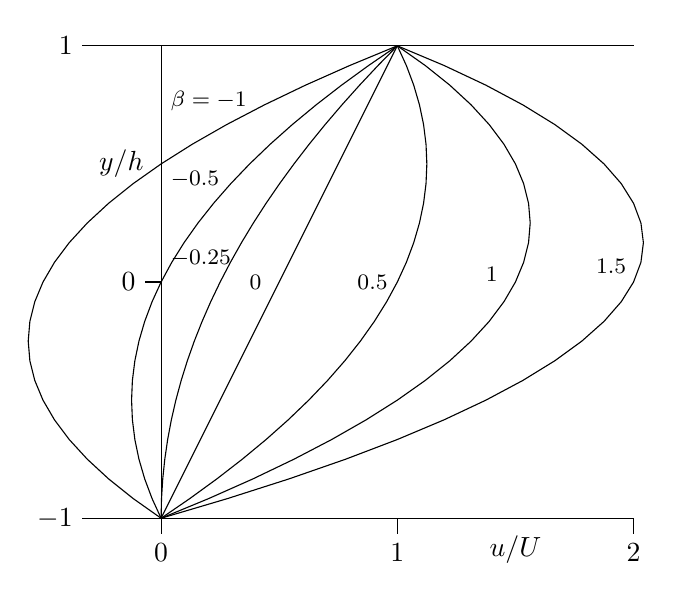
\begin{tikzpicture}
  \draw (-4,-3) -- (3,-3);
  \draw (-4,3) -- (3,3);
  \draw (-3,-3) -- (-3,3);
  \foreach \i in {0,...,2}
  {
    \pgfmathsetmacro{\x}{(-3 + \i*3)};
    \draw (\x,-3) -- ++(0,-0.2);
    \draw (\x,-3.2) node [below] {$\i$};
  }
  \draw (-3,0) -- ++(-0.2,0);
  \draw (-3.2,0) node [left] {$0$};
  \draw (-4,-3) node [left] {$-1$};
  \draw (-4,3) node [left] {$1$};
  \draw (1.5,-3.1) node [below] {$u/U$};
  \draw (-3.1, 1.5) node [left] {$y/h$};

  \foreach \i in {-1,-0.5,-0.25,0,0.5,1,1.5}
  {
    \draw [domain=-1:1] plot ({(\i*(1-(\x)^(2)) + 1/2*(1+\x))*3-3},{\x*3});
  }
  \draw (-3,2.3) node [right] {\footnotesize $\beta=-1$};
  \draw (-3,1.3) node [right] {\footnotesize $-0.5$};
  \draw (-3,0.3) node [right] {\footnotesize $-0.25$};
  \draw (-2,0) node [right] {\footnotesize $0$};
  \draw (0,0) node [left] {\footnotesize $0.5$};
  \draw (1,0.1) node [right] {\footnotesize $1$};
  \draw (2.4,0.2) [right] node {\footnotesize $1.5$};

\end{tikzpicture}

          \caption{Profil de vitesse pour l'écoulement de Poiseuille-Couette entre 2 plaques}
        \end{figure}

      \subsubsection{Écoulements axisymétriques}
        Soit un écoulement axisymétrique en conduite cylindrique de diamètre $D=2R$ (Hagen-Poiseuille).  Le repère est centré, avec $x$ la direction d'écoulement et $r$ la direction radiale.
        \begin{figure}[!h]
          \centering
          % !TEX root = ../meca1321-synthesis.tex
\tikzsetnextfilename{Hagen}
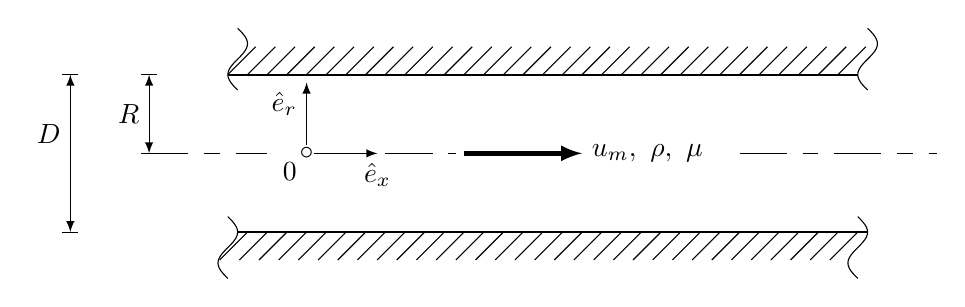
\begin{tikzpicture}
  % Tracé des parois
  \draw [thick] (-4,1) -- (4,1);
  \draw [domain=-pi:pi] plot ({sin(deg(\x))/8-3.875},{((\x+pi/2)/8+1});
  \draw [domain=-pi:pi] plot ({sin(deg(\x))/8+4.125},{((\x+pi/2)/8+1});
  \draw [thick] (-3.875,-1) -- (4.125,-1);
  \draw [domain=-pi:pi] plot ({sin(deg(\x))/8-4},{((\x-pi/2)/8-1});
  \draw [domain=-pi:pi] plot ({sin(deg(\x))/8+4},{((\x-pi/2)/8-1});
  \foreach \i in {0,...,31}
  {
    \pgfmathsetmacro{\x}{(- 4 + \i/4)};
    \draw (\x,1) -- ++(45:0.5);
    \draw (\x+1/4,-1) -- ++(-135:0.5);
  }
  %Repères et autres flèches
  \draw [dash pattern= on 0.6cm off 0.2cm on 0.2cm off 0.2cm] (-5.1,0) -- (-3.5,0);
  \draw [>=latex,<->] (-6,-1) -- (-6,1);
  \draw (-5.1,1) -- ++(0.2,0);
  \draw (-5,0.5) node [left] {$R$};
  \draw [>=latex,<->] (-5,0) -- (-5,1);
  \draw (-6.1,1) -- ++(0.2,0);
  \draw (-6.1,-1) -- ++(0.2,0);
  \draw (-6,0) node [above left] {$D$};
  \draw (-3,0) node {$\circ$};
  \draw (-3,0) node [below left] {$0$};
  \draw [>=latex,->] (-3,0.1) -- (-3,0.9);
  \draw [>=latex,->] (-2.9,0) -- (-2.1,0);
  \draw (-3.0,0.9) node [below left] {$\hat{\vb{e}}_r$};
  \draw (-2.1,0) node [below] {$\hat{\vb{e}}_x$};
  \draw [dash pattern= on 0.6cm off 0.2cm on 0.2cm off 0.2cm] (-2,0) -- (-1.1,0);
  \draw [ultra thick,>=latex,->] (-1,0) -- (0.5,0);
  \draw (0.5,0) node [right] {$u_m,~\rho,~\mu$};
  \draw [dash pattern= on 0.6cm off 0.2cm on 0.2cm off 0.2cm] (2.5,0) -- (5,0);
\end{tikzpicture}

          \caption{Écoulement établi en conduite}
          \label{fig:Hagen}
        \end{figure}
        Comme pour les écoulements plans, on a $u = u(r)$, $\pdv{u}{x} = 0$, $\pdv{r}(rv) = 0$ et $v = 0$. En reprenant l'équation de quantité de mouvement,
        \begin{equation}
          \begin{aligned}
            0 &= -\dv{P}{x} + \frac{\nu}{r} \dv{r}\left(r\dv{u}{r}\right)\\
            u(r) &= \dv{P}{x} \recip{\nu} \left(\frac{r^2}{4} + C_1 \log r + C_2 \right)\\
            u(r) &= - \dv{P}{x} \frac{R^2}{4\nu} \left(1 - \left(\frac{r}{R}\right)^2\right) = - \dv{p}{x} \frac{R^2}{4\mu} \left(1 - \left(\frac{r}{R}\right)^2\right)
          \end{aligned}
        \end{equation}

        On récupère alors les données comme précédemment:
        \begin{multicols}{2}
          \begin{equation*}
            u_c = -\dv{p}{x} \frac{R^2}{4\mu}
          \end{equation*}
          \begin{equation*}
            Q = \int_A u(r)dA = \frac{\pi R^2 u_c}{2}
          \end{equation*}

          \begin{equation*}
            u_m = \frac{Q}{A} = \frac{u_c}{2}
          \end{equation*}
          \begin{equation}
            u(r) = 2 u_m \left(1 - \left(\frac{r}{R}\right)^2\right)
          \end{equation}
        \end{multicols}
        La contrainte de frontement à la paroi et le coefficient de frottement sont
        \begin{multicols}{2}
          \begin{equation*}
            \tau_w = -\mu \dv{u}{r}\eval_{r=R} = \frac{4\mu u_m}{R}
          \end{equation*}

          \begin{equation*}
              C_f = \frac{2 \tau_w}{\rho u_m^2} = \frac{8\nu}{R u_m} = \frac{16}{Re_D}
          \end{equation*}
        \end{multicols}
        avec $Re_D = u_m D/\nu$ de l'écoulement ici basé sur la vitesse de débit et le diamètre de la conduite. Le coefficient de perte de charge est alors
        \begin{equation}
          \begin{aligned}
            \lambda &= - \frac{2D}{\rho u_m^2} \dv{p}{x}\\
            &= 4 C_f = \frac{64}{Re_D}
          \end{aligned}
        \end{equation}

        \begin{figure}[!h]
          \centering
          % !TEX root = meca1321-synthesis.tex
\tikzsetnextfilename{HagenProfile}
\begin{tikzpicture}[scale=0.8]
  \draw (-4,-3) -- (3,-3);
  \draw (-4,3) -- (3,3);
  \draw (-3,-3) -- (-3,3);
  \foreach \i in {0,...,2}
  {
    \pgfmathsetmacro{\x}{(-3 + \i*3)};
    \draw (\x,-3) -- ++(0,-0.2);
    \draw (\x,-3.2) node [below] {$\i$};
  }
  \draw (-3,0) -- ++(-0.2,0);
  \draw (-3.2,0) node [left] {$0$};
  \draw (-4,-3) node [left] {$-1$};
  \draw (-4,3) node [left] {$1$};
  \draw (1.5,-3.1) node [below] {$u/u_m$};
  \draw (-3.1, 1.5) node [left] {$r/R$};
  \draw [domain=-1:1] plot ({2*(1-(\x)^(2))*3-3},{\x*3});
\end{tikzpicture}

          \label{fig:HagenProfile}
          \caption{Profil de vitesse pour l'écoulement de Hagen entre 2 plaques}
        \end{figure}

  \section{Écoulements instationnaires}
    \subsection{Démarrage brusque de l'écoulement dans une conduite}
      Pour un écoulent instationnaire en conduite, il faut tenir compte du temps:
      \begin{equation}
        \pdv{u}{t} = -\dv{P}{x} + \nu \frac{1}{r} \pdv{r} \left(r\pdv{u}{r}\right) \label{eq:instat}
      \end{equation}
      On considère qu'en $t<0$, il n'y a pas de gradient de pression et donc $u(r, t<0) = 0$. Un gradient de pression est imposé à la conduit à partir de $t=0_+$, démarrant l'écoulement qui tend vers l'écoulement de Poiseuille en $t \rightarrow \infty$. On est donc face à un problème aux conditionx limites et initiales. On peut alors obtenir l' équation de la différence entre $u(r, t)$ et $u(r, t\rightarrow\infty)$, appelée $\tilde{u}(r,t)$, en soustrayant les équations \ref{eq:instat} et \ref{eq:Poiseuille}.
      \begin{equation}
        \pdv{\tilde{u}}{t} = \nu \frac{1}{r} \pdv{r} \left(r\pdv{\tilde{u}}{r}\right)
      \end{equation}
      avec comme condition initiale $\tilde{u}(r,0)=u_c\left(1-\left(\frac{r}{R}\right)^2\right)$ et comme condition limite $\tilde{u}(R,t)=0$. On adimensionnalise de la façon suivante
      \begin{equation}
        \begin{aligned}
          \tilde{u}^\ast = \frac{\tilde{u}}{u_c}, \quad \eta = \frac{r}{R}, \quad \zeta = \frac{\nu t}{R^2}\\
          \pdv{\tilde{u}^\ast}{\zeta} = \recip{\eta}\pdv{\eta}\left(\eta\pdv{\tilde{u}^\ast}{\eta}\right)
        \end{aligned}
      \end{equation}
      avec $\tilde{u}^\ast(\eta,0) = 1-\eta^2$ et $\tilde{u}^\ast(1, \zeta) = 0$. Le problème est séparable $\tilde{u}^\ast = f(\eta)g(\zeta)$. Le développement complet se trouve en page $38-39$ du syllabus mais la solution
      \begin{equation}
        \begin{aligned}
          \frac{u}{u_c} &= (1-\eta^2) - 8 \sum^\infty_{n=1} \frac{J_0(\lambda{n}\eta)}{\lambda_n^3 J_1(\lambda_n)}e^{-\lambda_n^2 \zeta}\\
          &= \left(1- \left(\frac{r}{R}\right)^2\right) - 8 \sum^\infty_{n=1} \frac{J_0\left(\lambda_n \frac{r}{R}\right)}{\lambda_n^3 J_1(\lambda_n)} \exp(-\lambda_n^2 \frac{\nu t}{R^2})
        \end{aligned}
      \end{equation}
      où $\lambda_n$ est la n\up{e} racine de la fonction de Bessel $J_0$
      \begin{figure}[!h]
        \centering
        % !TEX root=meca1321-synthesis.tex
\tikzsetnextfilename{instatio}
\begin{tikzpicture}
  \draw (-5,-3) -- (4,-3);
  \draw (-5,3) -- (4,3);
  \draw (-4,-3) -- (-4,3);
  \foreach \i in {0,...,1}
  {
    \pgfmathsetmacro{\x}{(-3 + \i*6)};
    \draw (\x,-3) -- ++(0,-0.2);
    \draw (\x,-3.2) node [below] {$\i$};
  }
  \draw (-4,0) -- ++(-0.2,0);
  \draw (-4.2,0) node [above left] {$0$};
  \draw (-5,-3) node [left] {$-1$};
  \draw (-5,3) node [left] {$1$};
  \draw (1.5,-3.1) node [below] {$u/u_c$};
  \draw (-4.1, 1.5) node [left] {$\eta$};
  \csvreader[ head to column names,%
                late after head=\xdef\aold{\a}\xdef\bold{\b},%
                after line=\xdef\aold{\a}\xdef\bold{\b}]%
                {instatio.csv}{}{%
    \draw (\bold*6-3, \aold*3) -- (\b*6-3,\a*3);
  }
  \csvreader[ head to column names,%
                late after head=\xdef\aold{\a}\xdef\cold{\c},%
                after line=\xdef\aold{\a}\xdef\cold{\c}]%
                {instatio.csv}{}{%
    \draw (\cold*6-3, \aold*3) -- (\c*6-3,\a*3);
  }
  \csvreader[ head to column names,%
                late after head=\xdef\aold{\a}\xdef\dold{\d},%
                after line=\xdef\aold{\a}\xdef\dold{\d}]%
                {instatio.csv}{}{%
    \draw (\dold*6-3, \aold*3) -- (\d*6-3,\a*3);
  }
  \csvreader[ head to column names,%
                late after head=\xdef\aold{\a}\xdef\eold{\e},%
                after line=\xdef\aold{\a}\xdef\eold{\e}]%
                {instatio.csv}{}{%
    \draw (\eold*6-3, \aold*3) -- (\e*6-3,\a*3);
  }
  \csvreader[ head to column names,%
                late after head=\xdef\aold{\a}\xdef\fold{\f},%
                after line=\xdef\aold{\a}\xdef\fold{\f}]%
                {instatio.csv}{}{%
    \draw (\fold*6-3, \aold*3) -- (\f*6-3,\a*3);
  }
  \csvreader[ head to column names,%
                late after head=\xdef\aold{\a}\xdef\gold{\g},%
                after line=\xdef\aold{\a}\xdef\gold{\g}]%
                {instatio.csv}{}{%
    \draw (\gold*6-3, \aold*3) -- (\g*6-3,\a*3);
  }
  \csvreader[ head to column names,%
                late after head=\xdef\aold{\a}\xdef\hold{\h},%
                after line=\xdef\aold{\a}\xdef\hold{\h}]%
                {instatio.csv}{}{%
    \draw (\hold*6-3, \aold*3) -- (\h*6-3,\a*3);
  }
  \draw (-3, 0) node [above left] {\footnotesize $\zeta=0$};
  \draw (-1.75, 0.05) node [above left] {\footnotesize $0.02$};
  \draw (-0.5, 0.05) node [above left] {\footnotesize $0.07$};
  \draw (1, 0.05) node [above left] {\footnotesize $0.15$};
  \draw (1.75, 0.05) node [above left] {\footnotesize $0.3$};
  \draw (2.95, 0.05) node [above left] {\footnotesize $0.8$};
  \draw (3, 0.05) node [above right] {\footnotesize $1$};
  \draw [dash pattern=on 3pt off 4pt on \the\pgflinewidth off 4pt] (-5, 0) -- (4, 0);
\end{tikzpicture}

      \end{figure}
      Le temps d'établissement d'un écoulement est donné par le terme exponentielle décroissant le moins rapidement ($\exp(-\lambda_1^2 \zeta)$). On peut donc utiliser comme temps caractéristique de développement\footnote{Temps pour passer de $1$ à $e^{-1}$} $\zeta_c \approx 1/\lambda^2_1$ (adimensionnel). Sur le long terme ($\zeta > \zeta_c$), on peut alors établir une estimation de $u$ au centre de la conduite
      \begin{equation}
        \frac{u}{u_c}(0, \zeta>\zeta_c) \approx 1 - \frac{8}{\lambda_1^3 J_1(\lambda_1)}e^{-\lambda_1\zeta}
      \end{equation}
      De là, les temps pour que la vitesse au centre soit égale à $95$ ou $99\%$ peuvent être obtenus.

      Il est possible d'établir un parallèle entre le démarrage brusque en conduite et la zone d'entrée d'un écoulement en conduite en considérant que celui-ci passe de $u(r)= u_m$ à l'écoulement de Poiseuille et en "remplaçant" $t_c$ par $x_c/u_m$. Cette analogie est cependant imparfaite et ne sera pas développée ici.

    \subsection{Écoulement cyclique avec gradient de pression oscillant}
      Considérons un gradient de pression oscillant à une fréquence circulaire $\omega$.
      \begin{equation}
        -\dv{P}{x} = -\dv{P}{x}\eval_0 \cos{\omega t} = -\dv{P}{x}\eval_0 e^{i\omega t}
      \end{equation}
      Bien entendu, on ne considère que la partie réelle. L'équation \ref{eq:Poiseuille}
      \begin{equation}
        \pdv{u}{t} = \frac{4\nu}{R^2} u_c e^{i\omega t} + \nu \recip{r}\pdv{r} \left(r\pdv{u}{r}\right)
      \end{equation}
      Les adimensionalisation à faire sont les suivantes
      \begin{equation}
        u^\ast = \frac{u}{u_c}, \quad \eta = \frac{r}{R}, \quad \omega^\ast = \frac{\omega R^2}{\nu}, \quad \zeta = \frac{t\nu}{R^2}
      \end{equation}
      La solution est de la forme
      \begin{equation}
        u^\ast = f(\eta) e^{i\omega^ast \zeta}
      \end{equation}
      Après résolution\footnote{Celle-ci se trouve page 43 du syllabus pour les plus curieux}, on obtient une solution générale
      \begin{equation}
        \frac{u}{u_c} = \real \left( \frac{4}{i\omega^\ast} \left( 1 - \frac{\Ber_0(\sqrt{\omega^\ast} \eta) + i \Bei_0(\sqrt{\omega^\ast} \eta)}{\Ber_0(\sqrt{\omega^\ast}) + i \Bei_0(\sqrt{\omega^\ast})} \right) e^{i\omega^\ast \zeta}\right)
      \end{equation}
      où $\Ber_0(s)$ et $\Bei_0(s)$ sont les parties réelles et imaginaires de la fonction de Bessel $J_0(e^{i3\pi/4}s)$. Cette solution est valable pour toutes les fréquences d'excitation. On distingue cependant deux cas particullier, les cas de forçages lent ($\sqrt{\omega^\ast}\eta$ est petit) et rapide ($\sqrt{\omega^\ast}\eta$ est grand).

      Dans le premier cas, on peut approximer $J_0(e^{i3\pi/4}s)$ via Taylor et obtenir
      \begin{equation}
        \begin{aligned}
          \frac{u}{u_c} &= \real \left(\left((1-\eta^2) - i \frac{\omega^\ast}{16} (\eta^4 - 4 \eta^2 +3) \right)e^{i\omega^\ast \zeta}\right)\\
          &= (1- \eta^2) \cos(\omega^\ast \zeta) + \frac{\omega^\ast}{16} (\eta^4 - 4 \eta^2 +3) \sin (\omega^\ast \zeta) + \mathcal{O}(\omega^{\ast2})
        \end{aligned}
      \end{equation}

      Dans le second, on utilise l'expansion asymptotique de $J_0(z)$ valable pour de grand $z$ pour obtenir
      \begin{equation}
        \begin{aligned}
          \frac{u}{u_c} &= \real \left(\frac{4}{i\omega^\ast}\left( \recip{\sqrt{\eta}}e^{-\sqrt{\frac{\omega^\ast}{2}}(1-\eta)} e^{-i \sqrt{\frac{\omega^\ast}{2}}(1-\eta)}\right)
          e^{i\omega^\ast \zeta}\right)\\
          &= \frac{4}{\omega^\ast} \left(\sin(\omega^\ast \zeta) - \recip{\sqrt{\eta}}e^{-\sqrt{\frac{\omega^\ast}{2}}(1-\eta)}\sin\left(\omega^\ast \zeta -\sqrt{\frac{\omega^\ast}{2}}(1-\eta) \right)
          \right) + \mathcal{O}\left(\recip{\omega^{\ast 2}}\right)
        \end{aligned}
      \end{equation}
      \begin{figure}[h]
        \centering
        \begin{minipage}[c]{0.45\textwidth}
          % !TEX root = ../meca1321-synthesis.tex
\tikzsetnextfilename{forcageLent}
\begin{tikzpicture}[scale=0.75]
  \draw (-4,-3) -- (4,-3);
  \draw (-4,3) -- (4,3);
  \draw (0,-3) -- (0,3);
  \draw [dash pattern=on 3pt off 4pt on \the\pgflinewidth off 4pt] (-4, 0) -- (4, 0);
  \foreach \i in {0,...,1}
  {
    \pgfmathsetmacro{\x}{(\i*3)};
    \draw (\x,-3) -- ++(0,-0.2);
    \draw (\x,-3.2) node [below] {$\i$};
  }
  \draw (-4,0) node [left] {$0$};
  \draw (-4,-3) node [left] {$-1$};
  \draw (-4,3) node [left] {$1$};
  \draw (1.5,-3.1) node [below] {$u/u_c$};
  \draw (-4.1, 1.5) node [left] {$\eta$};
  \csvreader[ head to column names,%
                late after head=\xdef\aold{\a}\xdef\bold{\b},%
                after line=\xdef\aold{\a}\xdef\bold{\b}]%
                {chapter2/forcageLent.csv}{}{%
    \draw (\bold*3, \aold*3) -- (\b*3,\a*3);
  }
  \csvreader[ head to column names,%
                late after head=\xdef\aold{\a}\xdef\cold{\c},%
                after line=\xdef\aold{\a}\xdef\cold{\c}]%
                {chapter2/forcageLent.csv}{}{%
    \draw (\cold*3, \aold*3) -- (\c*3,\a*3);
  }
  \csvreader[ head to column names,%
                late after head=\xdef\aold{\a}\xdef\dold{\d},%
                after line=\xdef\aold{\a}\xdef\dold{\d}]%
                {chapter2/forcageLent.csv}{}{%
    \draw (\dold*3, \aold*3) -- (\d*3,\a*3);
  }
  \csvreader[ head to column names,%
                late after head=\xdef\aold{\a}\xdef\eold{\e},%
                after line=\xdef\aold{\a}\xdef\eold{\e}]%
                {chapter2/forcageLent.csv}{}{%
                \draw (\eold*3, \aold*3) -- (\e*3,\a*3);
  }
  \draw (-2, 1.3) node  {\footnotesize $3\pi/4$};
  \draw (0.6, 1.3) node {\footnotesize $\pi/2$};
  \draw (1.9, 1.2) node [left] {\footnotesize $\pi/4$};
  \draw (2.5, 1.2) node [right] {\footnotesize $\zeta\omega^\ast = 0$};
\end{tikzpicture}

          \caption{Écoulement cyclique en cond-uite circulaire: cas d'un forçage lent ($\omega^\ast = 1/2$). Solution exacte.}
          \label{fig:forcageLent}
        \end{minipage}
        \begin{minipage}[c]{0.45\textwidth}
          % !TEX root = ../meca1321-synthesis.tex
\tikzsetnextfilename{forcageRapide}
\begin{tikzpicture}[scale=0.75]
  \draw (-4,-3) -- (4,-3);
  \draw (-4,3) -- (4,3);
  \draw (-3,-3) -- (-3,3);
  \draw [dash pattern=on 3pt off 4pt on \the\pgflinewidth off 4pt] (-4, 0) -- (4, 0);
  \foreach \i in {0,0.25}
  {
    \pgfmathsetmacro{\x}{(\i*6*4-3)};
    \draw (\x,-3) -- ++(0,-0.2);
    \draw (\x,-3.2) node [below] {$\i$};
  }
  \draw (-4,0) node [left] {$0$};
  \draw (-4,-3) node [left] {$-1$};
  \draw (-4,3) node [left] {$1$};
  \draw (1.5,-3.1) node [below] {$u/u_c$};
  \draw (-4.1, 1.5) node [left] {$\eta$};
  \csvreader[ head to column names,%
                late after head=\xdef\aold{\a}\xdef\bold{\b},%
                after line=\xdef\aold{\a}\xdef\bold{\b}]%
                {chapter2/forcageRapide.csv}{}{%
    \draw (\bold*6*4-3, \aold*3) -- (\b*6*4-3,\a*3);
  }
  \csvreader[ head to column names,%
                late after head=\xdef\aold{\a}\xdef\cold{\c},%
                after line=\xdef\aold{\a}\xdef\cold{\c}]%
                {chapter2/forcageRapide.csv}{}{%
    \draw (\cold*6*4-3, \aold*3) -- (\c*6*4-3,\a*3);
  }
  \csvreader[ head to column names,%
                late after head=\xdef\aold{\a}\xdef\dold{\d},%
                after line=\xdef\aold{\a}\xdef\dold{\d}]%
                {chapter2/forcageRapide.csv}{}{%
    \draw (\dold*6*4-3, \aold*3) -- (\d*6*4-3,\a*3);
  }
  \csvreader[ head to column names,%
                late after head=\xdef\aold{\a}\xdef\eold{\e},%
                after line=\xdef\aold{\a}\xdef\eold{\e}]%
                {chapter2/forcageRapide.csv}{}{%
                \draw (\eold*6*4-3, \aold*3) -- (\e*6*4-3,\a*3);
  }
  \draw (-1.5, 0.5) node  {\footnotesize $\zeta\omega^\ast = 0$};
  \draw (0, 1.7) node {\footnotesize $3\pi/4$};
  \draw (2.5, 0.4) node [left] {\footnotesize $\pi/4$};
  \draw (2.5, 1.2) node [right] {\footnotesize $\pi/2$};
\end{tikzpicture}

          \caption{Écoulement cyclique en cond-uite circulaire: cas d'un forçage rapide ($\omega^\ast = 20$). Solution exacte.}
          \label{fig:forcageRapide}
        \end{minipage}
      \end{figure}

    \subsection{Démarrage brusque d'une plaque}
      Comme une plaque ne bloque l'écoulent d'un côté\footnote{L'autre côté est considéré infini}, il n'y a pas de gradient de pression latéral. On a donc
      \begin{equation}
        \pdv{u}{t} = \nu \pdv[2]{u}{y}
      \end{equation}
      qui est l'équation de diffusion. La plaque démarre en $t=0_+$ à une vitesse $U$. On a $\eta = y/2\sqrt{\nu t}$ et
      \begin{equation}
        \frac{u}{U} = f\left(\frac{y}{2\sqrt{\nu t}}\right) = f(\eta)
      \end{equation}
      Après résolution,  on a
      \begin{equation}
        \frac{u}{U} = 1 - \frac{2}{\sqrt{\pi}}\int_0^\eta e^{\eta'^2} d\eta'  = 1-\erf(\eta) = \erfc(\eta)
      \end{equation}
      où $\erf$ est la fonction erreur et $\erfc$ est la fonction erreur complémentaire.
      Le tourbillon est également obtenu via
      \begin{equation}
        \omega = -\pdv{u}{y} = U \frac{2}{\pi} e^{-\eta^2} \frac{1}{2\sqrt{\nu t}} = \frac{U}{\sqrt{\pi\nu t}}e^{-\frac{y^2}{4\nu t}}
      \end{equation}

      \begin{figure}[!h]
        \centering
        \begin{minipage}[c]{0.45\textwidth}
          % !TEX root=meca1321-synthesis.tex
\tikzsetnextfilename{demarPlaqueVitesse}
\begin{tikzpicture}
  \draw (-2, -2.5) -- (2, -2.5);
  \draw (-2, -2.5) -- (-2, 2.5);
  \foreach \i in {0,2,...,10}
  {
    \pgfmathsetmacro{\x}{(\i/2)};
    \draw (-2, \x-2.5) -- ++(-0.2, 0);
    \draw (-2.2, \x-2.5) node [left] {$\i$};
  }
  \foreach \i in {0, 1}
  {
    \draw (\i*4-2, -2.5) -- ++ (0, -0.2);
    \draw (\i*4-2, -2.7) node [below] {$\i$};
  }
  \csvreader[ head to column names,%
                late after head=\xdef\aold{\a}\xdef\bold{\b},%
                after line=\xdef\aold{\a}\xdef\bold{\b}]%
                {demarPlaqueVitesse.csv}{}{%
    \draw (\bold*4-2, \aold/2-2.5) -- (\b*4-2,\a/2-2.5);
  }
  \csvreader[ head to column names,%
                late after head=\xdef\aold{\a}\xdef\cold{\c},%
                after line=\xdef\aold{\a}\xdef\cold{\c}]%
                {demarPlaqueVitesse.csv}{}{%
    \draw (\cold*4-2, \aold/2-2.5) -- (\c*4-2,\a/2-2.5);
  }
  \csvreader[ head to column names,%
                late after head=\xdef\aold{\a}\xdef\dold{\d},%
                after line=\xdef\aold{\a}\xdef\dold{\d}]%
                {demarPlaqueVitesse.csv}{}{%
    \draw (\dold*4-2, \aold/2-2.5) -- (\d*4-2,\a/2-2.5);
  }
  \csvreader[ head to column names,%
                late after head=\xdef\aold{\a}\xdef\eold{\e},%
                after line=\xdef\aold{\a}\xdef\eold{\e}]%
                {demarPlaqueVitesse.csv}{}{%
    \draw (\eold*4-2, \aold/2-2.5) -- (\e*4-2,\a/2-2.5);
  }
  \draw (-1.7,-2.35) node {\footnotesize $0.5$};
  \draw (-1.6,-1.7) node {\footnotesize $1$};
  \draw (-1.3,-1.3) node {\footnotesize $2$};
  \draw (-0.5,0) node {\footnotesize $2\sqrt{\nu t} = 5$};
  \draw (-3, 2) node [left] {$y$};
  \draw (1, -2.5) node [below] {$\frac{u}{U}$};
\end{tikzpicture}

          \label{fig:demarPlaqueVitesse}
        \end{minipage}
        \begin{minipage}[c]{0.45\textwidth}
          % !TEX root = ../meca1321-synthesis.tex
\tikzsetnextfilename{demarPlaqueTourb}
\begin{tikzpicture}
    \draw (-2, -2.5) -- (2.5, -2.5);
    \draw (-2, -2.5) -- (-2, 2.5);
    \foreach \i in {0,2,...,10}
    {
      \pgfmathsetmacro{\x}{(\i/2)};
      \draw (-2, \x-2.5) -- ++(-0.2, 0);
      \draw (-2.2, \x-2.5) node [left] {$\i$};
    }
    \foreach \i in {0,...,2}
    {
      \draw (\i*2-2, -2.5) -- ++ (0, -0.2);
      \draw (\i*2-2, -2.7) node [below] {$\i$};
    }
    \csvreader[ head to column names,%
                  late after head=\xdef\aold{\a}\xdef\bold{\b},%
                  after line=\xdef\aold{\a}\xdef\bold{\b}]%
                  {chapter2/demarPlaqueTourb.csv}{}{%
      \draw (\bold*2-2, \aold/2-2.5) -- (\b*2-2,\a/2-2.5);
    }
    \csvreader[ head to column names,%
                  late after head=\xdef\aold{\a}\xdef\cold{\c},%
                  after line=\xdef\aold{\a}\xdef\cold{\c}]%
                  {chapter2/demarPlaqueTourb.csv}{}{%
      \draw (\cold*2-2, \aold/2-2.5) -- (\c*2-2,\a/2-2.5);
    }
    \csvreader[ head to column names,%
                  late after head=\xdef\aold{\a}\xdef\dold{\d},%
                  after line=\xdef\aold{\a}\xdef\dold{\d}]%
                  {chapter2/demarPlaqueTourb.csv}{}{%
      \draw (\dold*2-2, \aold/2-2.5) -- (\d*2-2,\a/2-2.5);
    }
    \csvreader[ head to column names,%
                  late after head=\xdef\aold{\a}\xdef\eold{\e},%
                  after line=\xdef\aold{\a}\xdef\eold{\e}]%
                  {chapter2/demarPlaqueTourb.csv}{}{%
      \draw (\eold*2-2, \aold/2-2.5) -- (\e*2-2,\a/2-2.5);
    }
    \draw (-0.7, -1.9) node {\footnotesize $1$};
    \draw (-1.2, -1.6) node {\footnotesize $2$};
    \draw (-1.7, 0) node {\footnotesize $5$};
    \draw (1.5, -2.2) node {\footnotesize $0.5$};
    \draw (-3, 2) node [left] {$y$};
    \draw (1, -2.5) node [below] {$\frac{\omega}{U}$};
\end{tikzpicture}

          \label{fig:demarPlaqueTourb}
        \end{minipage}
        \caption{Démarrage brusque d'une plaque: développement des profils de vitesse et de tourbillon}
      \end{figure}

    \subsection{Plaque oscillante}
      Dans le cas d'une plaque oscillante, la vitesse est
      \begin{equation}
        U cos(\omega t) = \real(U e^{i\omega t})
      \end{equation}
      On utilise $\eta = y \sqrt{\frac{\omega}{\nu}}$, ce qui nous donne
      \begin{equation}
        \dv[2]{f}{\eta} - i f = 0
      \end{equation}
      et
      \begin{equation}
        \frac{u}{U} = \real\left(e^{-\recip{\sqrt{2}}(1+i)\eta}e^{i\omega t}\right)
        = e^{-\frac{\eta}{\sqrt{2}}}\cos\left(\omega t-\frac{\eta}{\sqrt{2}}\right)
        = e^{-y \sqrt{\frac{\omega}{2\nu}}} \cos\left(\omega t - y\frac{\omega}{2\nu}\right)
      \end{equation}
      L'amplitude de la vitesse décroit de manière exponentielle. De plus, elle est déphasée par rapport à la plaque proportionnellement à la distance à la plaque $\phi = y\frac{\omega}{2\nu}$

      \begin{figure}[!h]
        \centering
        % !TEX root=meca1321-synthesis.tex
\tikzsetnextfilename{plaqueOsci}
\begin{tikzpicture}
  \draw (-3, 3) -- (-3, -3);
  \draw (-3, -3) -- (3, -3);
  \draw (3, 3) -- (3, -3);
  \foreach \i in {0, 2,..., 6}
  {
    \draw (-3.2, \i-3) node [left] {$\i$};
    \draw (-3, \i-3) -- ++(-0.2, 0);
  }
  \foreach \i in {-1,0,1}
  {
    \draw (\i*3, -3.2) node [below] {$\i$};
    \draw (\i*3, -3) -- ++(0, -0.2);
  }
  \csvreader[ head to column names,%
                late after head=\xdef\aold{\a}\xdef\bold{\b},%
                after line=\xdef\aold{\a}\xdef\bold{\b}]%
                {plaqueOsci.csv}{}{%
    \draw (\bold*3, \aold-3) -- (\b*3,\a-3);
  }
  \csvreader[ head to column names,%
                late after head=\xdef\aold{\a}\xdef\cold{\c},%
                after line=\xdef\aold{\a}\xdef\cold{\c}]%
                {plaqueOsci.csv}{}{%
    \draw (\cold*3, \aold-3) -- (\c*3,\a-3);
  }
  \csvreader[ head to column names,%
                late after head=\xdef\aold{\a}\xdef\dold{\d},%
                after line=\xdef\aold{\a}\xdef\dold{\d}]%
                {plaqueOsci.csv}{}{%
    \draw (\dold*3, \aold-3) -- (\d*3,\a-3);
  }
  \csvreader[ head to column names,%
                late after head=\xdef\aold{\a}\xdef\eold{\e},%
                after line=\xdef\aold{\a}\xdef\eold{\e}]%
                {plaqueOsci.csv}{}{%
    \draw (\eold*3, \aold-3) -- (\e*3,\a-3);
  }
  \csvreader[ head to column names,%
                late after head=\xdef\aold{\a}\xdef\fold{\f},%
                after line=\xdef\aold{\a}\xdef\fold{\f}]%
                {plaqueOsci.csv}{}{%
    \draw (\fold*3, \aold-3) -- (\f*3,\a-3);
  }
  \csvreader[ head to column names,%
                late after head=\xdef\aold{\a}\xdef\gold{\g},%
                after line=\xdef\aold{\a}\xdef\gold{\g}]%
                {plaqueOsci.csv}{}{%
    \draw (\gold*3, \aold-3) -- (\g*3,\a-3);
  }
  \csvreader[ head to column names,%
                late after head=\xdef\aold{\a}\xdef\hold{\h},%
                after line=\xdef\aold{\a}\xdef\hold{\h}]%
                {plaqueOsci.csv}{}{%
    \draw (\hold*3, \aold-3) -- (\h*3,\a-3);
  }
  \draw (2.8, -2.7) node {\footnotesize $0$};
  \draw (2, -2.2) node {\footnotesize $\pi/6$};
  \draw (1.3, -2.7) node {\footnotesize $\pi/3$};
  \draw (0.6, -2.5) node {\footnotesize $\pi/2$};
  \draw (-0.2, -2.8) node {\footnotesize $2\pi/3$};
  \draw (-1.7, -2.9) node {\footnotesize $5\pi/6$};
  \draw (-2, -2.3) node {\footnotesize $\omega t = \pi$};
\end{tikzpicture}

        \caption{Oscillation d'une plaque: profils de vitesse}
        \label{fig:plaqueOsci}
      \end{figure}

  \section{Zone d'entrée et longueur d'établissement}
    Un écoulement entrant dans une conduite de diamètre invariable ne s'établit pas immédiatement. À l'entrée, on a un écoulement bouchon qui devient progressivement un écoulement Poiseuille. On considère qu'il faut au moins une longueur d'établissement $x_c$ importante pour voir un ce dernier apparaître.

    Les équations qui régissent le problème d'établissement sont celles de la couche limite
    \begin{equation}
      \begin{aligned}
        \pdv{u}{x} + \recip{r} \pdv{r}(rv) &= 0\\
        u\pdv{u}{x} + v \pdv{u}{r} &= -\dv{P}{x} + \nu \recip{r} \pdv{r}\left(r\pdv{u}{r}\right)
      \end{aligned}
    \end{equation}
    Dans ce cas, la pression n'est fonction que de $x$ est négligeable par rapport à $r$. Une couche limite se développe ici le long de la paroi et son épaisseur $\delta(x)$ grandit selon $x$ jusqu'à atteindre le centre en $x = x_c$. A partir de là, on un profil de Poiseuille\footnote{D'un point de vue mathématique, l'évolution de $\delta(x)$ est asymptotique. On utilise donc $x_{c,0.95}$ ou $x_{c,0.99}$ qui représente le $x$ où la vitesse au centre est à $95\%$ ou $99\%$ de la vitesse maximale}.

    La pression $P(x) = p(x)/\rho$ est déterminée par la vitesse d'écoulement hors de la couche limite. Dans cette partie irrotationnelle, l'équation de Bernoulli dit
    \begin{equation}
      \begin{aligned}
        P(x) +\recip{2} u_c^2(x) &= cste = P(0) + \recip{2}u_m^2\\
        \dv{P}{x} + u_c \dv{u_c}{x} &=0
      \end{aligned}
    \end{equation}
    Ce qui nous donne
    \begin{equation}
      \begin{aligned}
        \pdv{u}{x} + \recip{r} \pdv{r}(rv) &= 0\\
        u\pdv{u}{x} + v \pdv{u}{r} &= u_c \dv{u_c}{x} + \nu \recip{r} \pdv{r}\left(r\pdv{u}{r}\right)
      \end{aligned}
    \end{equation}
    avec $u(0, r) = u_m$ et $u(x, R)= 0$.

    \textit{In fine}, le problème ci-dessus n'a pas de solution analytique, seulement numérique. Cependant, on peut établir que la loi régissant la longueur d'établissement est de la forme
    \begin{equation}
      \frac{x_c}{D} = f\left(\frac{u_m D}{\nu}\right) = f(Re_D)
    \end{equation}
